Good teaching requires good preparation.  The first step in preparing to teach in Tanzania it to create a Scheme of Work. This document helps you to lay out your lessons for the year, so that you will be able to cover all topics in the syllabus in a timely manner with remaining time to review.  Many people may tell you to copy the syllabus as the scheme of work, but this is a waste of time and in no way beneficial to you.  Instead, take a day and lay out your plans for the year.   Cater your Scheme of Work to your needs and the needs of your students. Below is a sample of the heading columns in a scheme of work. Remember, you should edit this document, adding or subtracting columns, in a way that makes sense to you.

\begin{flushleft}
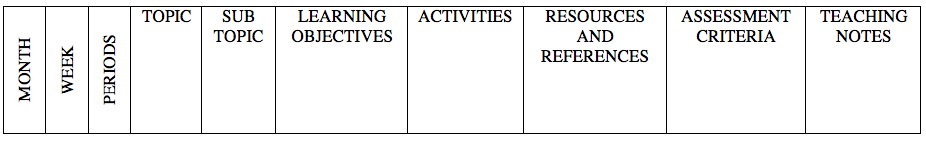
\includegraphics[scale=.4]{picture-1.jpg} 
\end{flushleft}


\section{How to Begin}
First, choose the topic in your subject you would like to begin the year with.  You may decide to follow the syllabus and teach the topics in the order the Ministry has outlined or you may decide to create your own order, choosing to teach the most important or relevant topic first.  Then, list the remaining topics in that subject and the order in which you would like to teach them.  Next, list the subtopics in each of those topics, again changing the order of the subtopics as you see fit.\\

\pagebreak
\begin{flushleft}
\begin{small}
For Example:\\
Biology Form IV\\
\textbf{1.0 Classification of Living Things\\}
1.1 Kingdom Animalia\\
1.1.1 Phylum Platyhelinthe\\
1.1.2 Phylum Aschelminthes (Nematoda)\\
1.1.3 Phylum Annelida\\
1.1.4 Phylum Arthropoda\\
1.1.5 Phylum Chordata\\
\textbf{2.0 Growth\\}
2.1 Concept of Growth\\
2.2 Mitosis and Growth\\
2.3 Growth and Development in Human Beings\\
2.4 Growth in Flowering Plants\\
\textbf{3.0 Genetics\\}
3.1 Concept of Genetics\\
3.2 Genetic Materials\\
3.3 Concept of Inheritance\\
3.3.2 Mendelian Inheritance\\
3.3.3 Non-Mendelian Inheritance\\
3.4 Sex Determination and Inheritance\\
3.5 Variation among Organisms\\
3.6 Genetic Disorders \\
3.7 Application of Genetics\\
\textbf{4.0 Evolution\\}
4.1 Concept of Organic Evolution\\
4.2 Theories of the Origin of Life\\
4.3 Theories of Organic Evolution\\
4.4 Evidence of Organic Evolution\\
\textbf{5.0 HIV, AIDS, and STIs\\}
5.1 Relationship between HIV, AIDs, and STIs\\
5.2 Management and Control of HIV/AIDs and STIs\\
5.3 Counseling and Voluntary Testing \\
\end{small}
\end{flushleft}

\section{Time Frame}
Now consider the amount of time it will take you to teach each of these topics and their subtopics. Use the syllabus while you are doing this.  Consider what the objectives are for each subtopic and how long it will take you to accomplish these objectives.  Consider the student background education as well.  For example, if you are teaching a topic in physics, maybe you want to add a period to review the mathematics required.  You may use the timetable in the syllabus as a guide, but you know your students better than the average time allotted by the Ministry of Education.  Each period is allocated a different amount of time per week.  Refer to the table below to determine how many periods a week your subject is allocated.\\

\begin{center}

\begin{tabular}{|c|c|c|}
\hline \rule[-2ex]{0pt}{5.5ex} Subject & Form & Periods per Week \\ 
\hline \rule[-2ex]{0pt}{5.5ex} Biology & 1,2 & 3 \\ 
\hline \rule[-2ex]{0pt}{5.5ex} Biology & 3,4 & 4 \\ 
\hline \rule[-2ex]{0pt}{5.5ex} Biology & 5,6 & 10 \\ 
\hline \rule[-2ex]{0pt}{5.5ex} Chemistry & 1,2 & 3 \\ 
\hline \rule[-2ex]{0pt}{5.5ex} Chemistry & 3,4  & 4 \\ 
\hline \rule[-2ex]{0pt}{5.5ex} Chemistry & 5,6 & 10 \\ 
\hline \rule[-2ex]{0pt}{5.5ex} Physics & 1,2 & 3 \\ 
\hline \rule[-2ex]{0pt}{5.5ex} Physics & 3,4 & 4 \\ 
\hline \rule[-2ex]{0pt}{5.5ex} Physics & 5,6 & 10 \\ 
\hline \rule[-2ex]{0pt}{5.5ex} Mathematics & 1-4 & 6 \\ 
\hline \rule[-2ex]{0pt}{5.5ex} Mathematics & 5,6  & 10 \\ 
\hline \rule[-2ex]{0pt}{5.5ex} English & 1-4 & 6 \\ 
\hline 
\end{tabular} 

\end{center}
Therefore, your Scheme of Work should now look something like this:

\begin{flushleft}
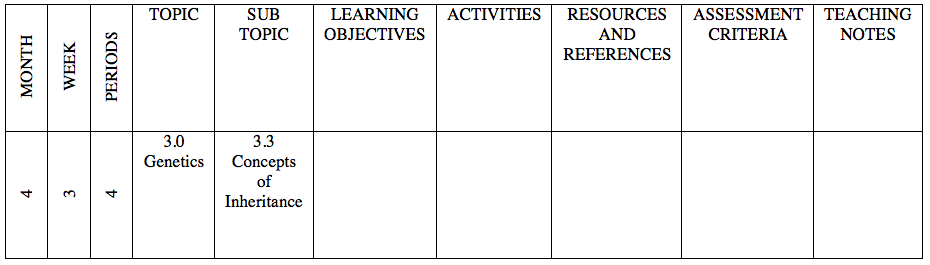
\includegraphics[scale=.4]{picture-2.jpg} 
\end{flushleft}

\section{Learning Objectives}
These are taken from the syllabus and are the one thing you can copy and paste directly.  Read each one of the corresponding subtopics and be sure the amount of time you have allocated for that subtopic is sufficient to meet these objectives.  You can reword or add objectives to this list as you see fit.

\section{Activities}
Now comes the hard work: brainstorming for future lessons.  This will be a great reference when it comes time to write your lesson plans.  In this column, list possible activities for you and your students to complete during class to meet the learning objectives for the subtopic.  Be creative here.  These ideas are not set in stone, but rather possibilities for interactive teaching.  This column may be broken into two columns as well; Teacher's Activities and Students' Activities. It is up to your discretion whether you would like to combine the two or keep them separate. At this point, you Scheme of Work should appear as follows:

\begin{flushleft}
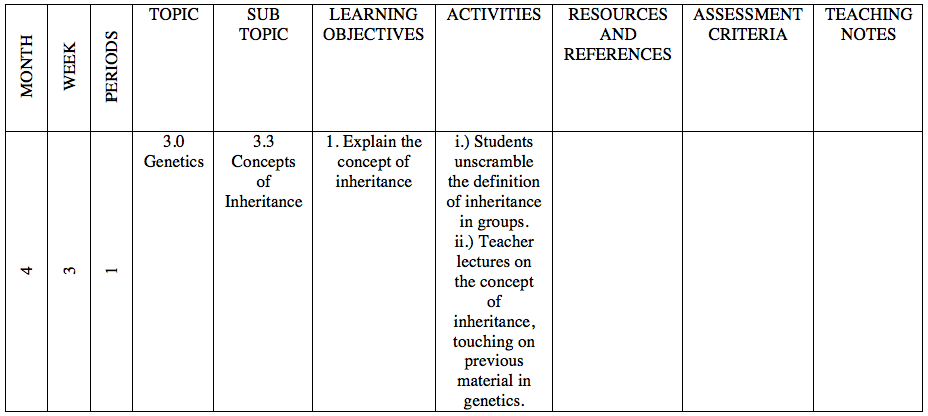
\includegraphics[scale=.4]{picture-3.jpg} 
\end{flushleft}

\section{Resources and References / Teaching Aids}
Review your activities in the previous column.  What materials or academic references do you need to make these activities a success?  You can include websites or reference books and their page numbers here, as well as any resources you might need to complete labs or games.

\section{Assessment Criteria}
This column is one of the most beneficial in the future when you are creating quizzes, assignments, and tests.  How will you know if your students have in fact reached the objectives for that subtopic?  This assessment criteria can be phrased in the form of a question or statement, but should be specific and reflect your lessons.  Consider the types of questions asked on NECTA, rather than referring to the very general assessment criteria in the syllabus.\\
Some examples: 
\begin{itemize}
\item Students can name the three states of matter and give an example of each
\item Students can calculate the volume of a cylinder from a word problem
\item Students will be able to list 5 advantages and 5 disadvantages of Kingdom Fungi
\end{itemize}
  

\section{Teaching Notes or Remarks}
This column will be left blank for observation or changes you may have in the future.  If a subtopic took longer to teach than you allocated, note this for next year.  It is possible you may want to change the topic order, or you found certain activities that worked well or not at all.  These will be noted in the Teaching Notes column after you have taught those lessons.  
Thus your final Scheme of Work will appear as follows:

\begin{flushleft}
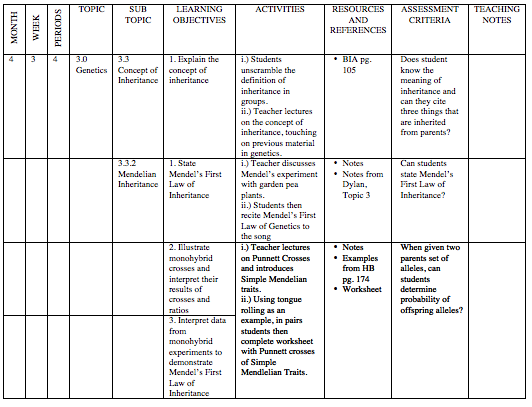
\includegraphics[scale=.7]{picture-4.jpg} 
\end{flushleft}

Creating a Scheme of Work may seem tedious or bureaucratic but it makes creating lesson plans and tests much easier.  A good Scheme of Work will keep your instruction organized and ensure that you have covered all topics and objectives with your students.  The Ministry of Education also requires it.   Try creating a document that is actually useful to you, rather than spending hours copying one that is not.
